\chapter{Конструкторская часть}

\section{Требования к программному обеспечению}
Программа должна предоставлять пользователю графический интерфейс, позволяющий:
\begin{itemize}
    \item загрузить исходный и целевой объект из \textit{.obj} файла;
    \item изменить цвет и оптические свойства поверхности загруженных объектов;
    \item просматривать по отдельности каждый объект и результат морфинга посредством поворота и масштабирования;
    \item изменять масштабирование и поворот исходного и целевого объектов морфинга;
    \item выбирать стадию морфинга объектов.
\end{itemize}

Программа должна корректно реагировать на любые действия пользователя.

\section{Используемы типы и структуры данных}
\begin{enumerate}
    \item[1)] Сцена состоит из:
    \begin{itemize}
        \item объекта;
        \item камеры;
        \item источника света.
    \end{itemize}

    \item[2)] Объект состоит из:
    \begin{itemize}
        \item массива точек;
        \item массива треугольников (индексы вершин);
        \item массива единичных внешних нормалей к треугольникам;
        \item материала;
        \item матрицы преобразований.
    \end{itemize}

    \item[3)] Результат морфинга, состоит из:
    \begin{itemize}
        \item массива точек;
        \item массива функций, интерполирующих вершины в момент $t$;
        \item массива треугольников (индексы вершин);
        \item массива единичных внешних нормалей к треугольникам;
        \item массива функций, интерполирующих внешние нормали в момент $t$;
        \item материала;
        \item функции интерполирующей материал в момент $t$;
        \item матрицы преобразований.
    \end{itemize}

%   TODO: пересмотреть состав камеры
    \item[4)] камера состоит из:
    \begin{itemize}
        \item положения;
        \item точки, на которую направлен взгляд;
        \item угол обзора в радианах;
        \item отношение сторон;
        \item уаление ближней плоскости пирамиды видимости;
        \item удаление дальней плоскости пирамды видимости.
    \end{itemize}

    \item[5)] источник света состоит из:
    \begin{itemize}
        \item положения;
        \item интесивности;
        % \item цвета; TODO: возможно убрать
    \end{itemize}

    \item[6)] материал состоит из:
    \begin{itemize}
        \item цвета в формате \textit{RGB};
        \item коэффициента диффузного отражения;
        \item коэффициента зеркального отражения;
        \item степени, аппроксимирующей пространственное распределение зеркально отраженного света.
    \end{itemize}
\end{enumerate}

Для построения суперсетки используется структура данных DCEL (doubly connected edge list)~\cite{alexa}.
Визуальное представление структуры данных приведено на рисунке~\ref{fig:DCEL}.

\begin{figure}[H]
    \centering
    \includegraphics[width=0.5\textwidth]{DCEL}
    \caption{DCEL (doubly connected edge list)~\cite{alexa}}
    \label{fig:DCEL}
\end{figure}

DCEL состоит из:

\begin{itemize}
    \item массива вершин;
    \item массива полуребер;
    \item массива граней;
\end{itemize}

Полуребро состоит из:
\begin{itemize}
    \item индекса вершины-начала;
    \item индекса полуребра-двойника;
    \item индекса смежной грани;
    \item индекса следующего полуребра;
\end{itemize}

Грань состоит из индекса полуребра, связанного с ней.

\section{Описание алгоритмов}

\begin{figure}[H]
    \includegraphics[width=\textwidth]{morphing_idef0}
    \caption{Функциональная диаграмма первого уровня, описывающая процесс построения морфинга}
    \label{fig:morphig_idef0}
\end{figure}

Схемы основных алгоритмов, используемых в программном обеспечены представлены на рисунках~\ref{fig:flowchart-z-buff}--\ref{fig:flowchart_normals_relocation}.

\begin{figure}[H]
    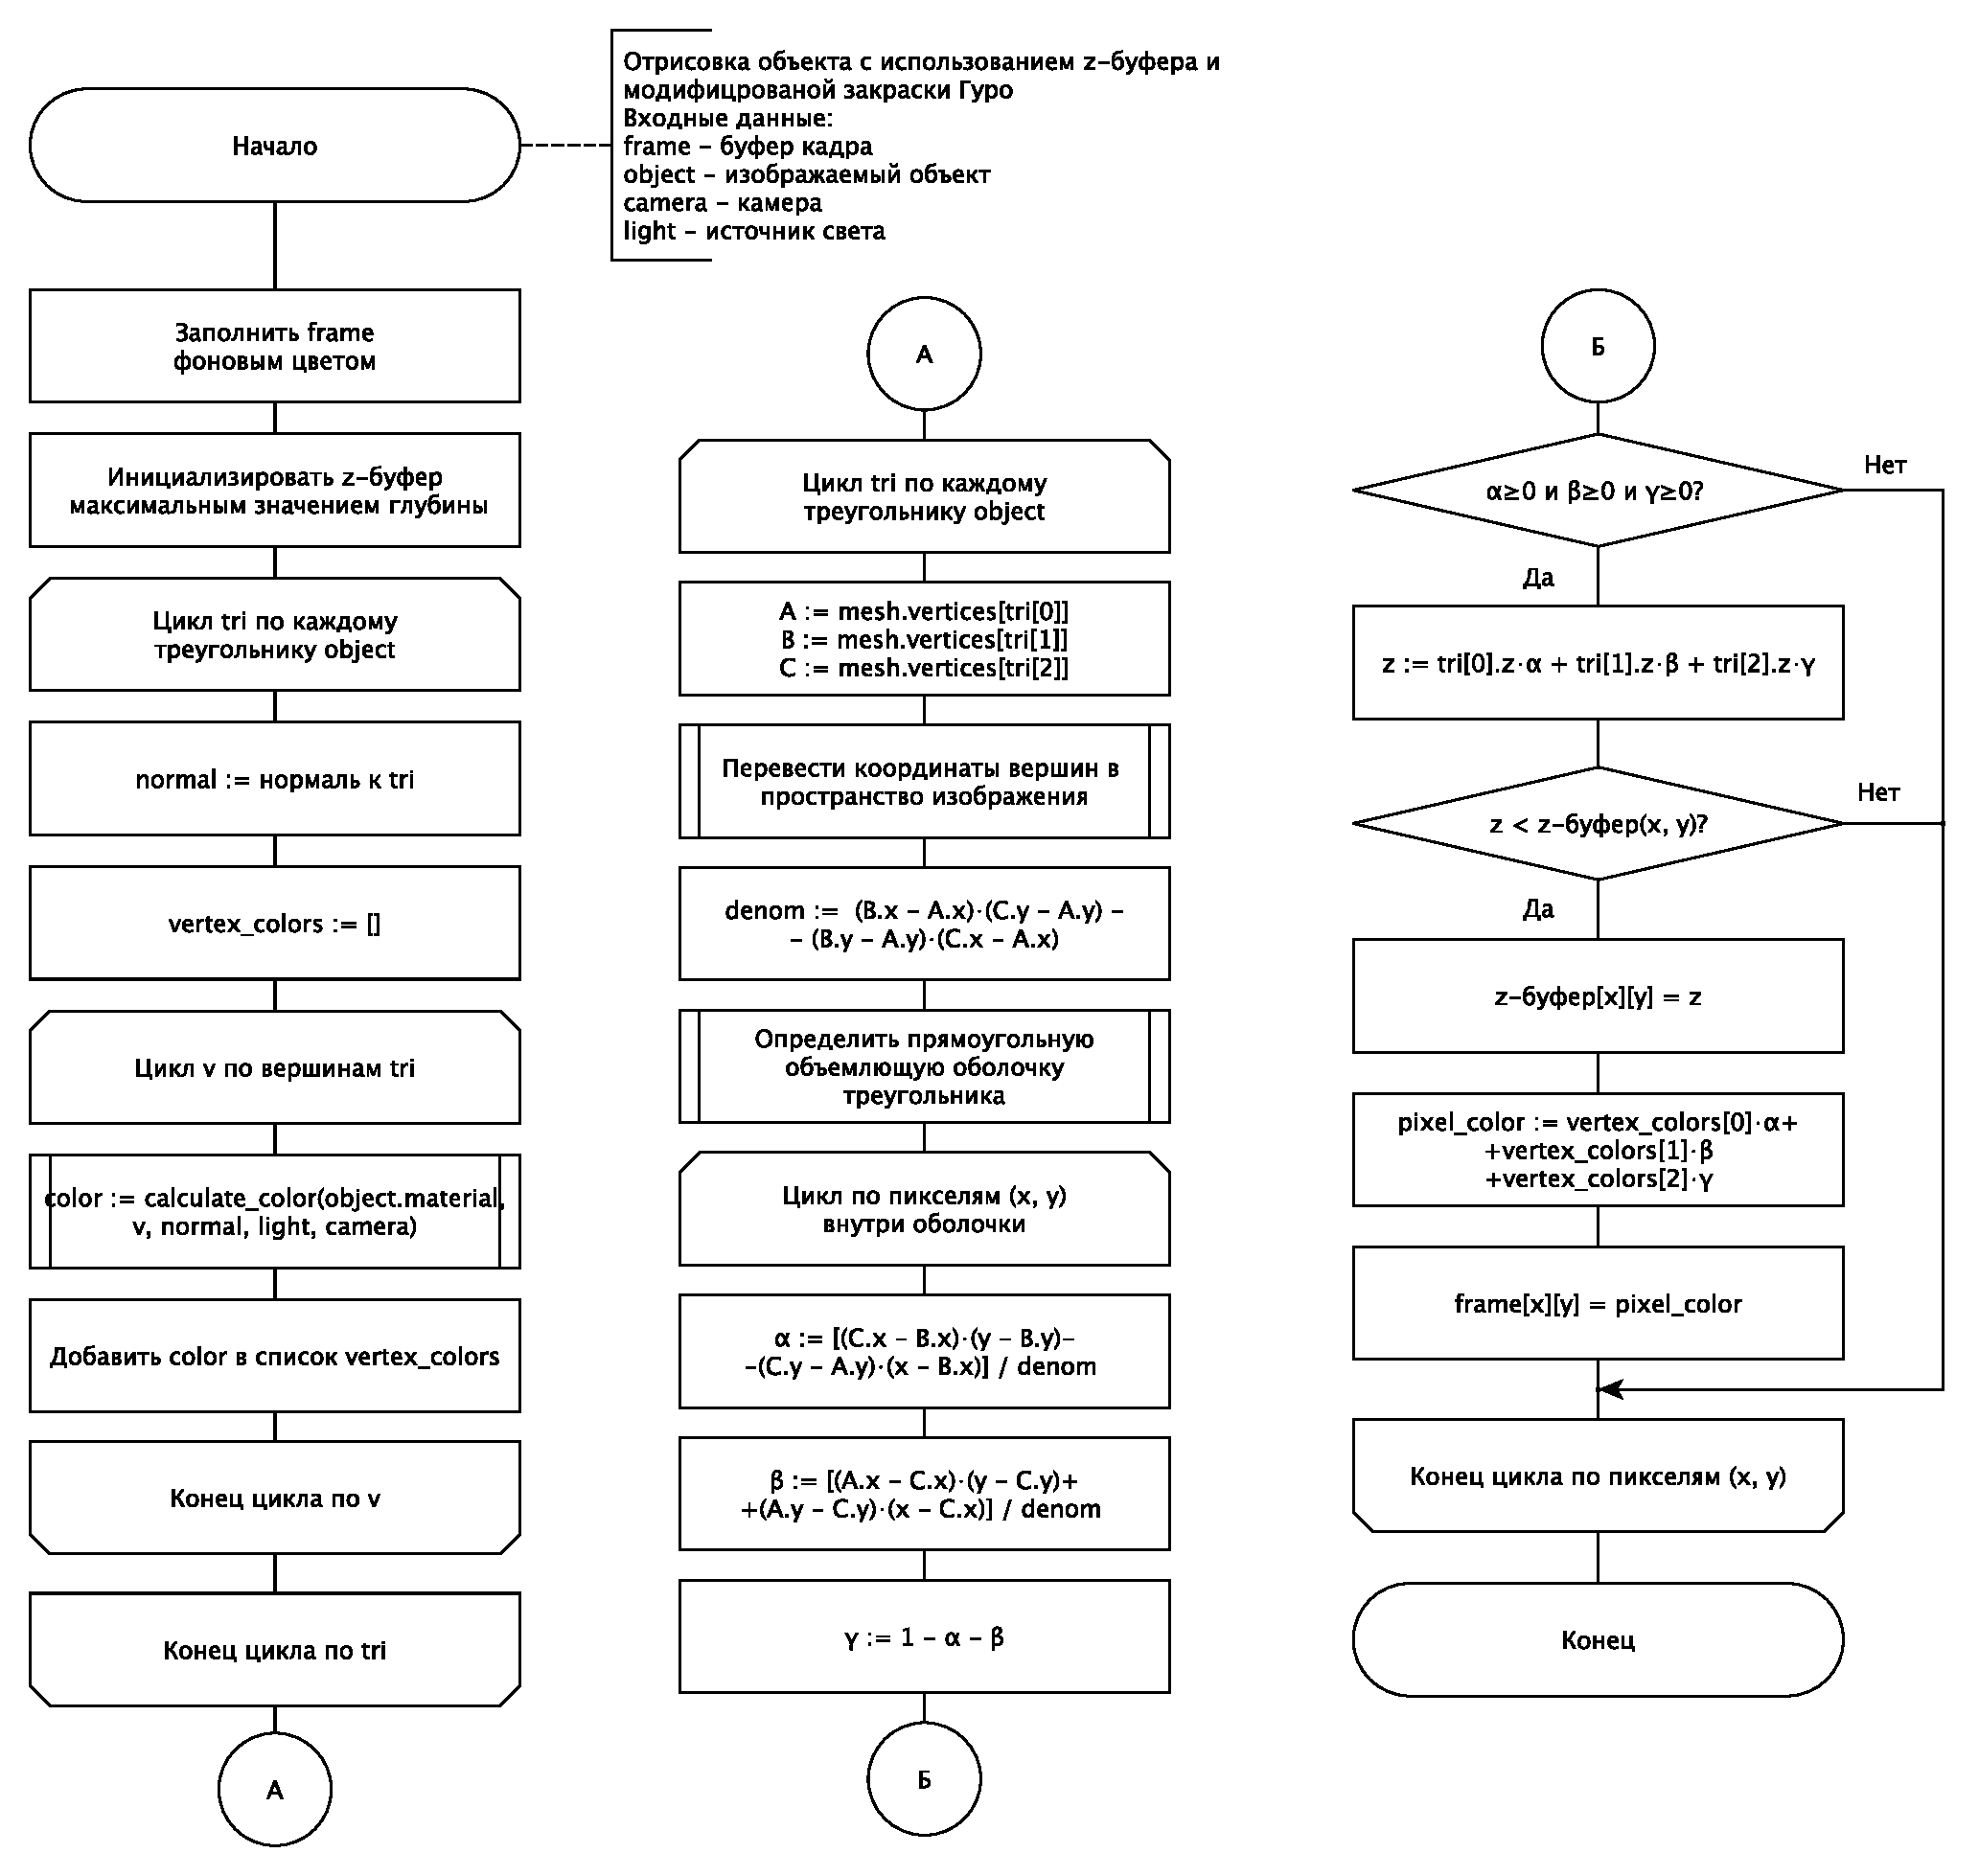
\includegraphics[width=\textwidth]{flowchart_z-buff}
    \caption{Схема алгоритма отрисовки объекта с использованием \textit{z}-буфера и модифицированной закраски Гуро}
    \label{fig:flowchart-z-buff}
\end{figure}

\begin{figure}[H]
    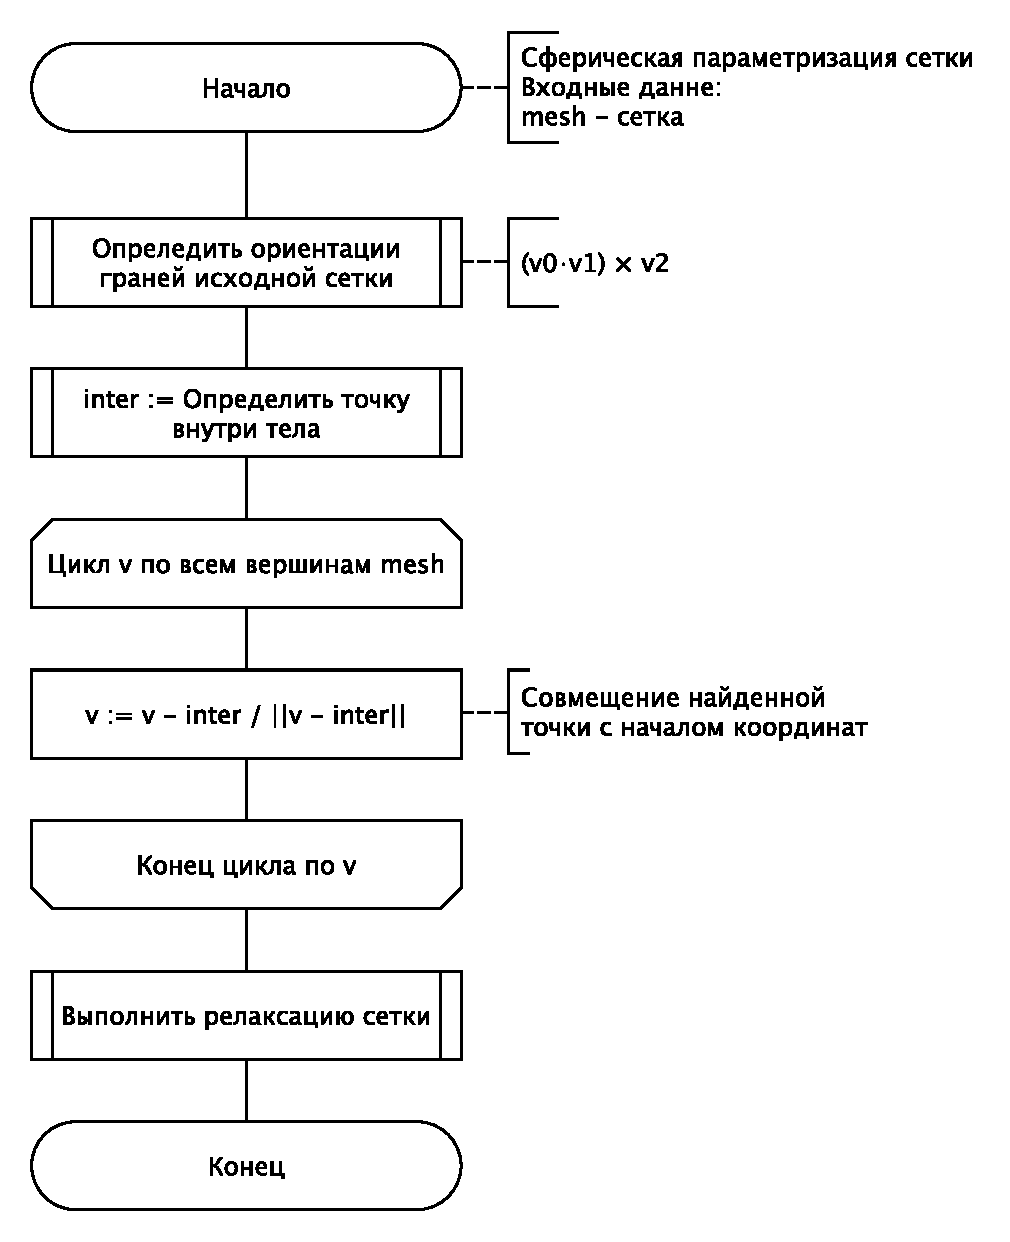
\includegraphics[width=\textwidth]{flowchart_parametriztion}
    \caption{Схема алгоритма сферической параметризации сетки}
    \label{fig:flowchart_parametrization}
\end{figure}

\begin{figure}[H]
    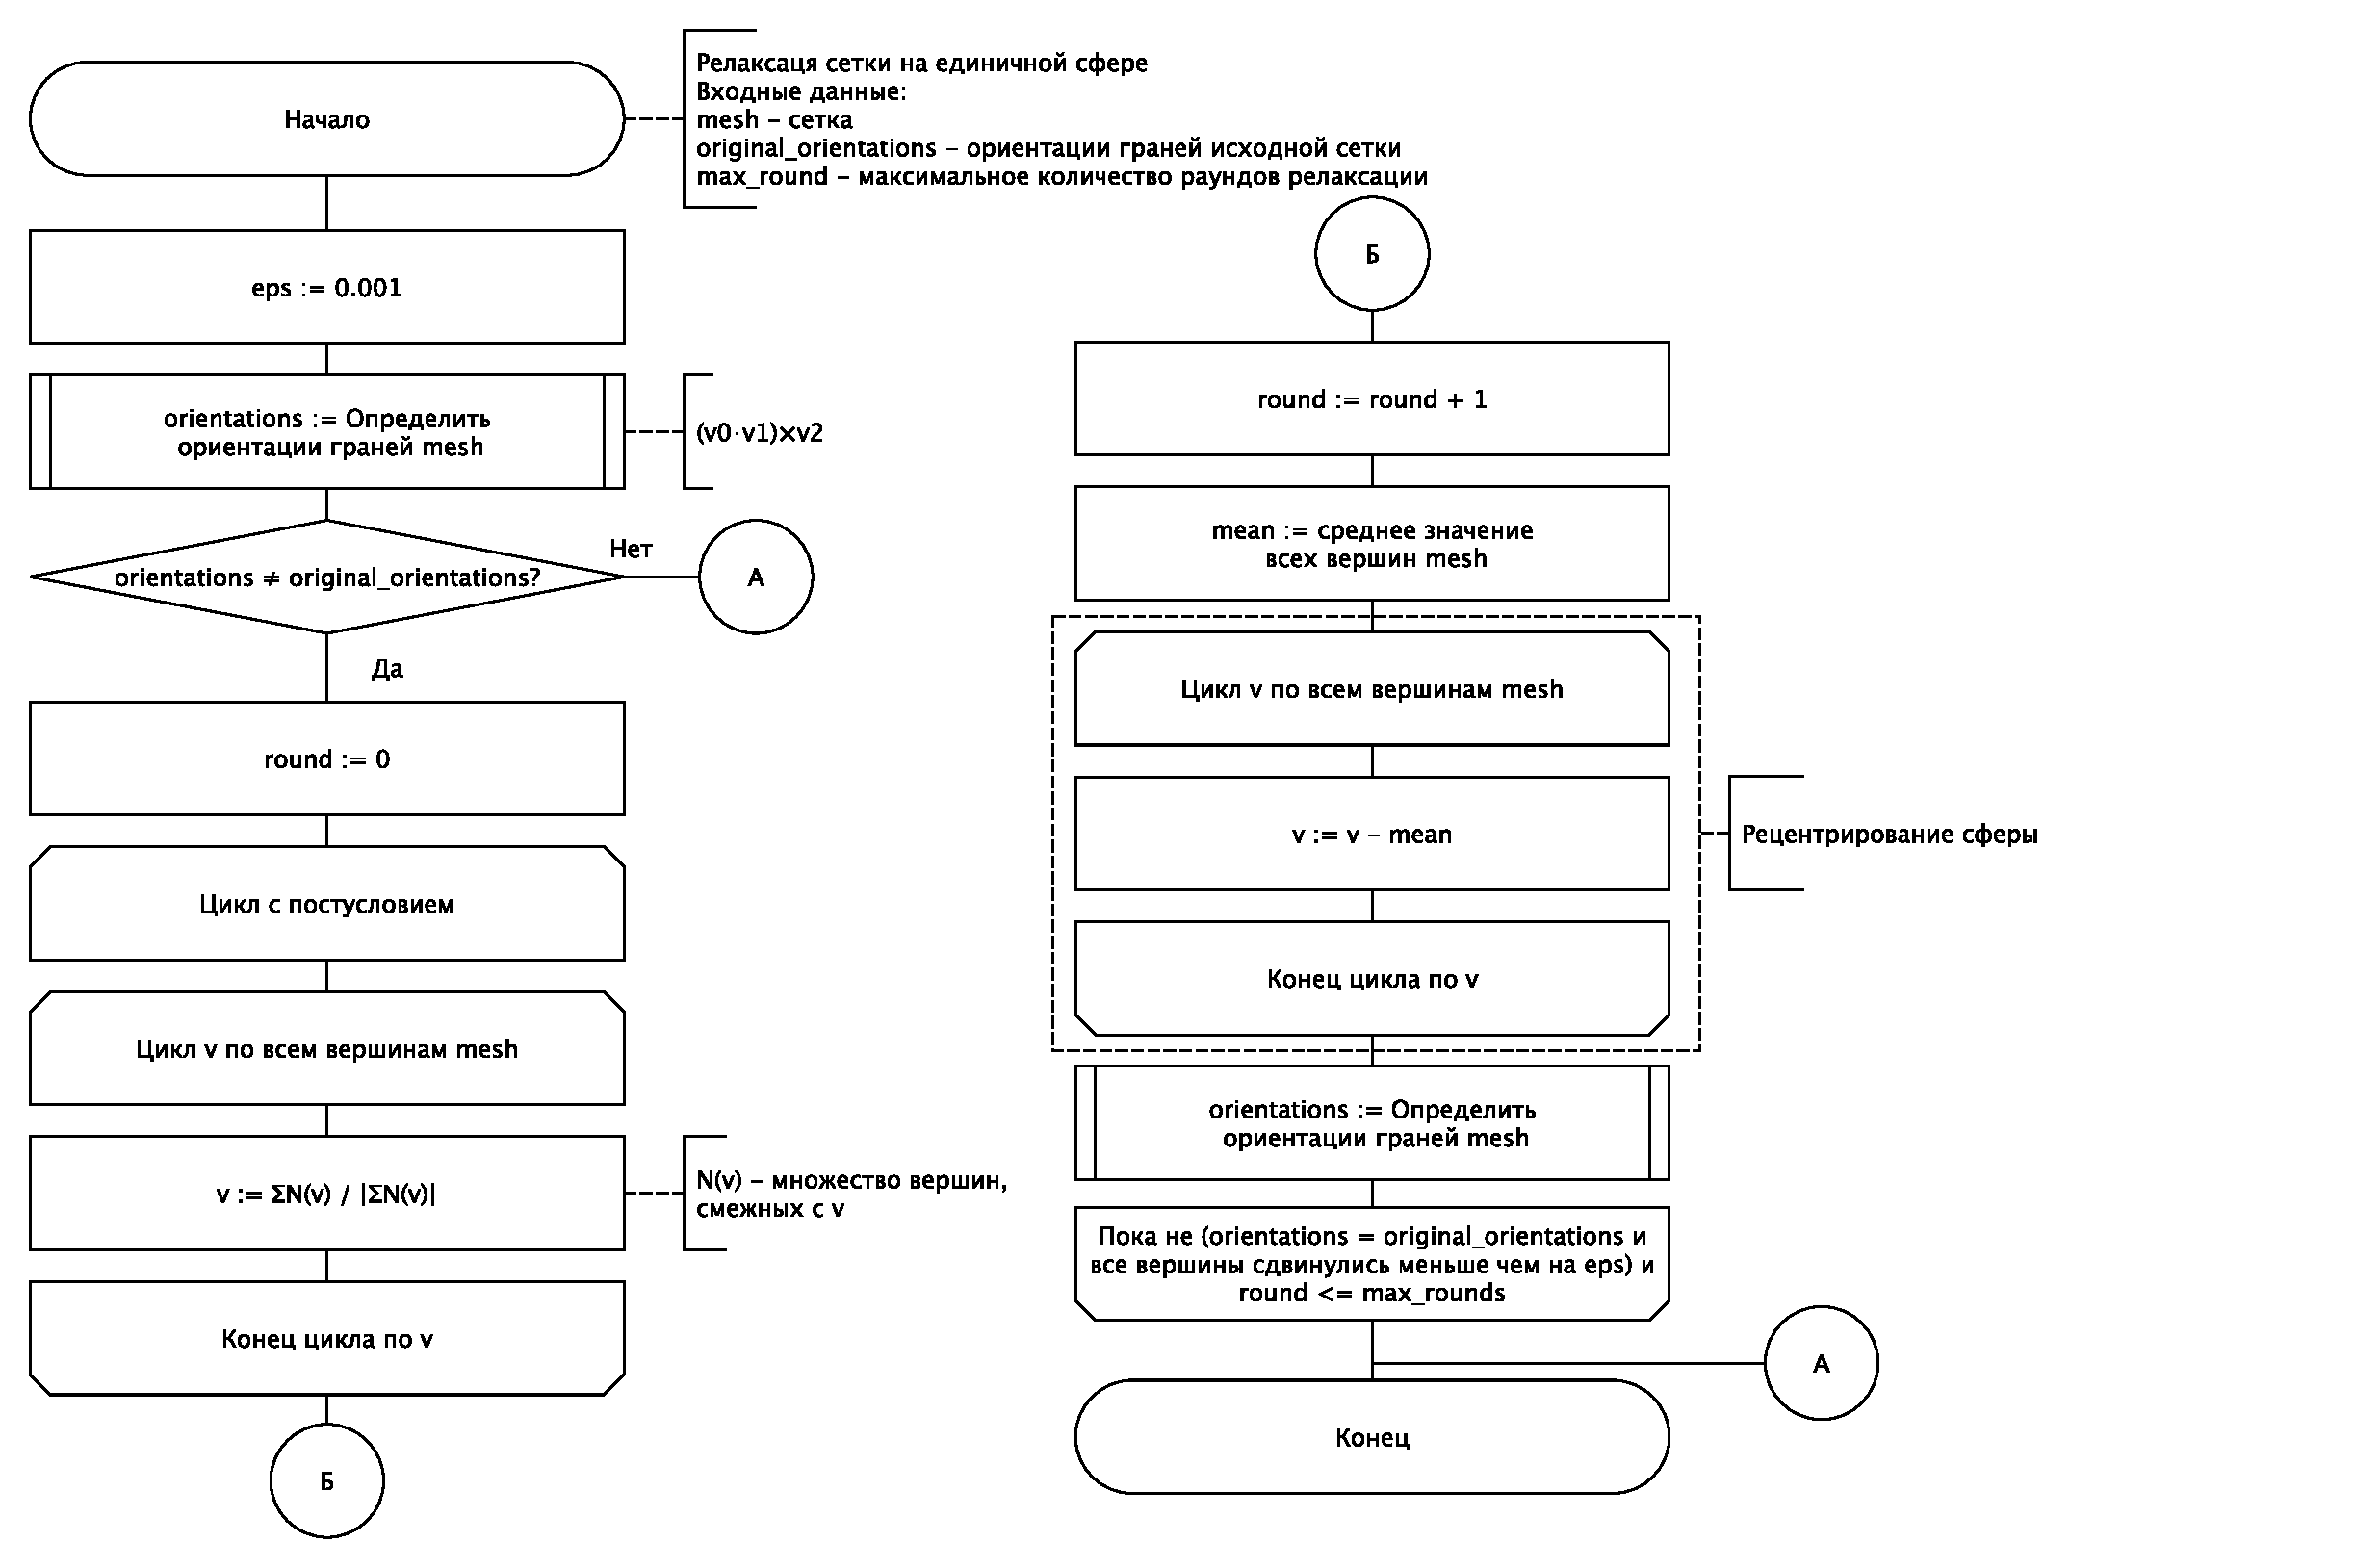
\includegraphics[width=\textwidth]{flowchart_relaxation}
    \caption{Схема алгоритма релаксации сетки}
    \label{fig:flowchart_relaxation}
\end{figure}

\begin{figure}[H]
    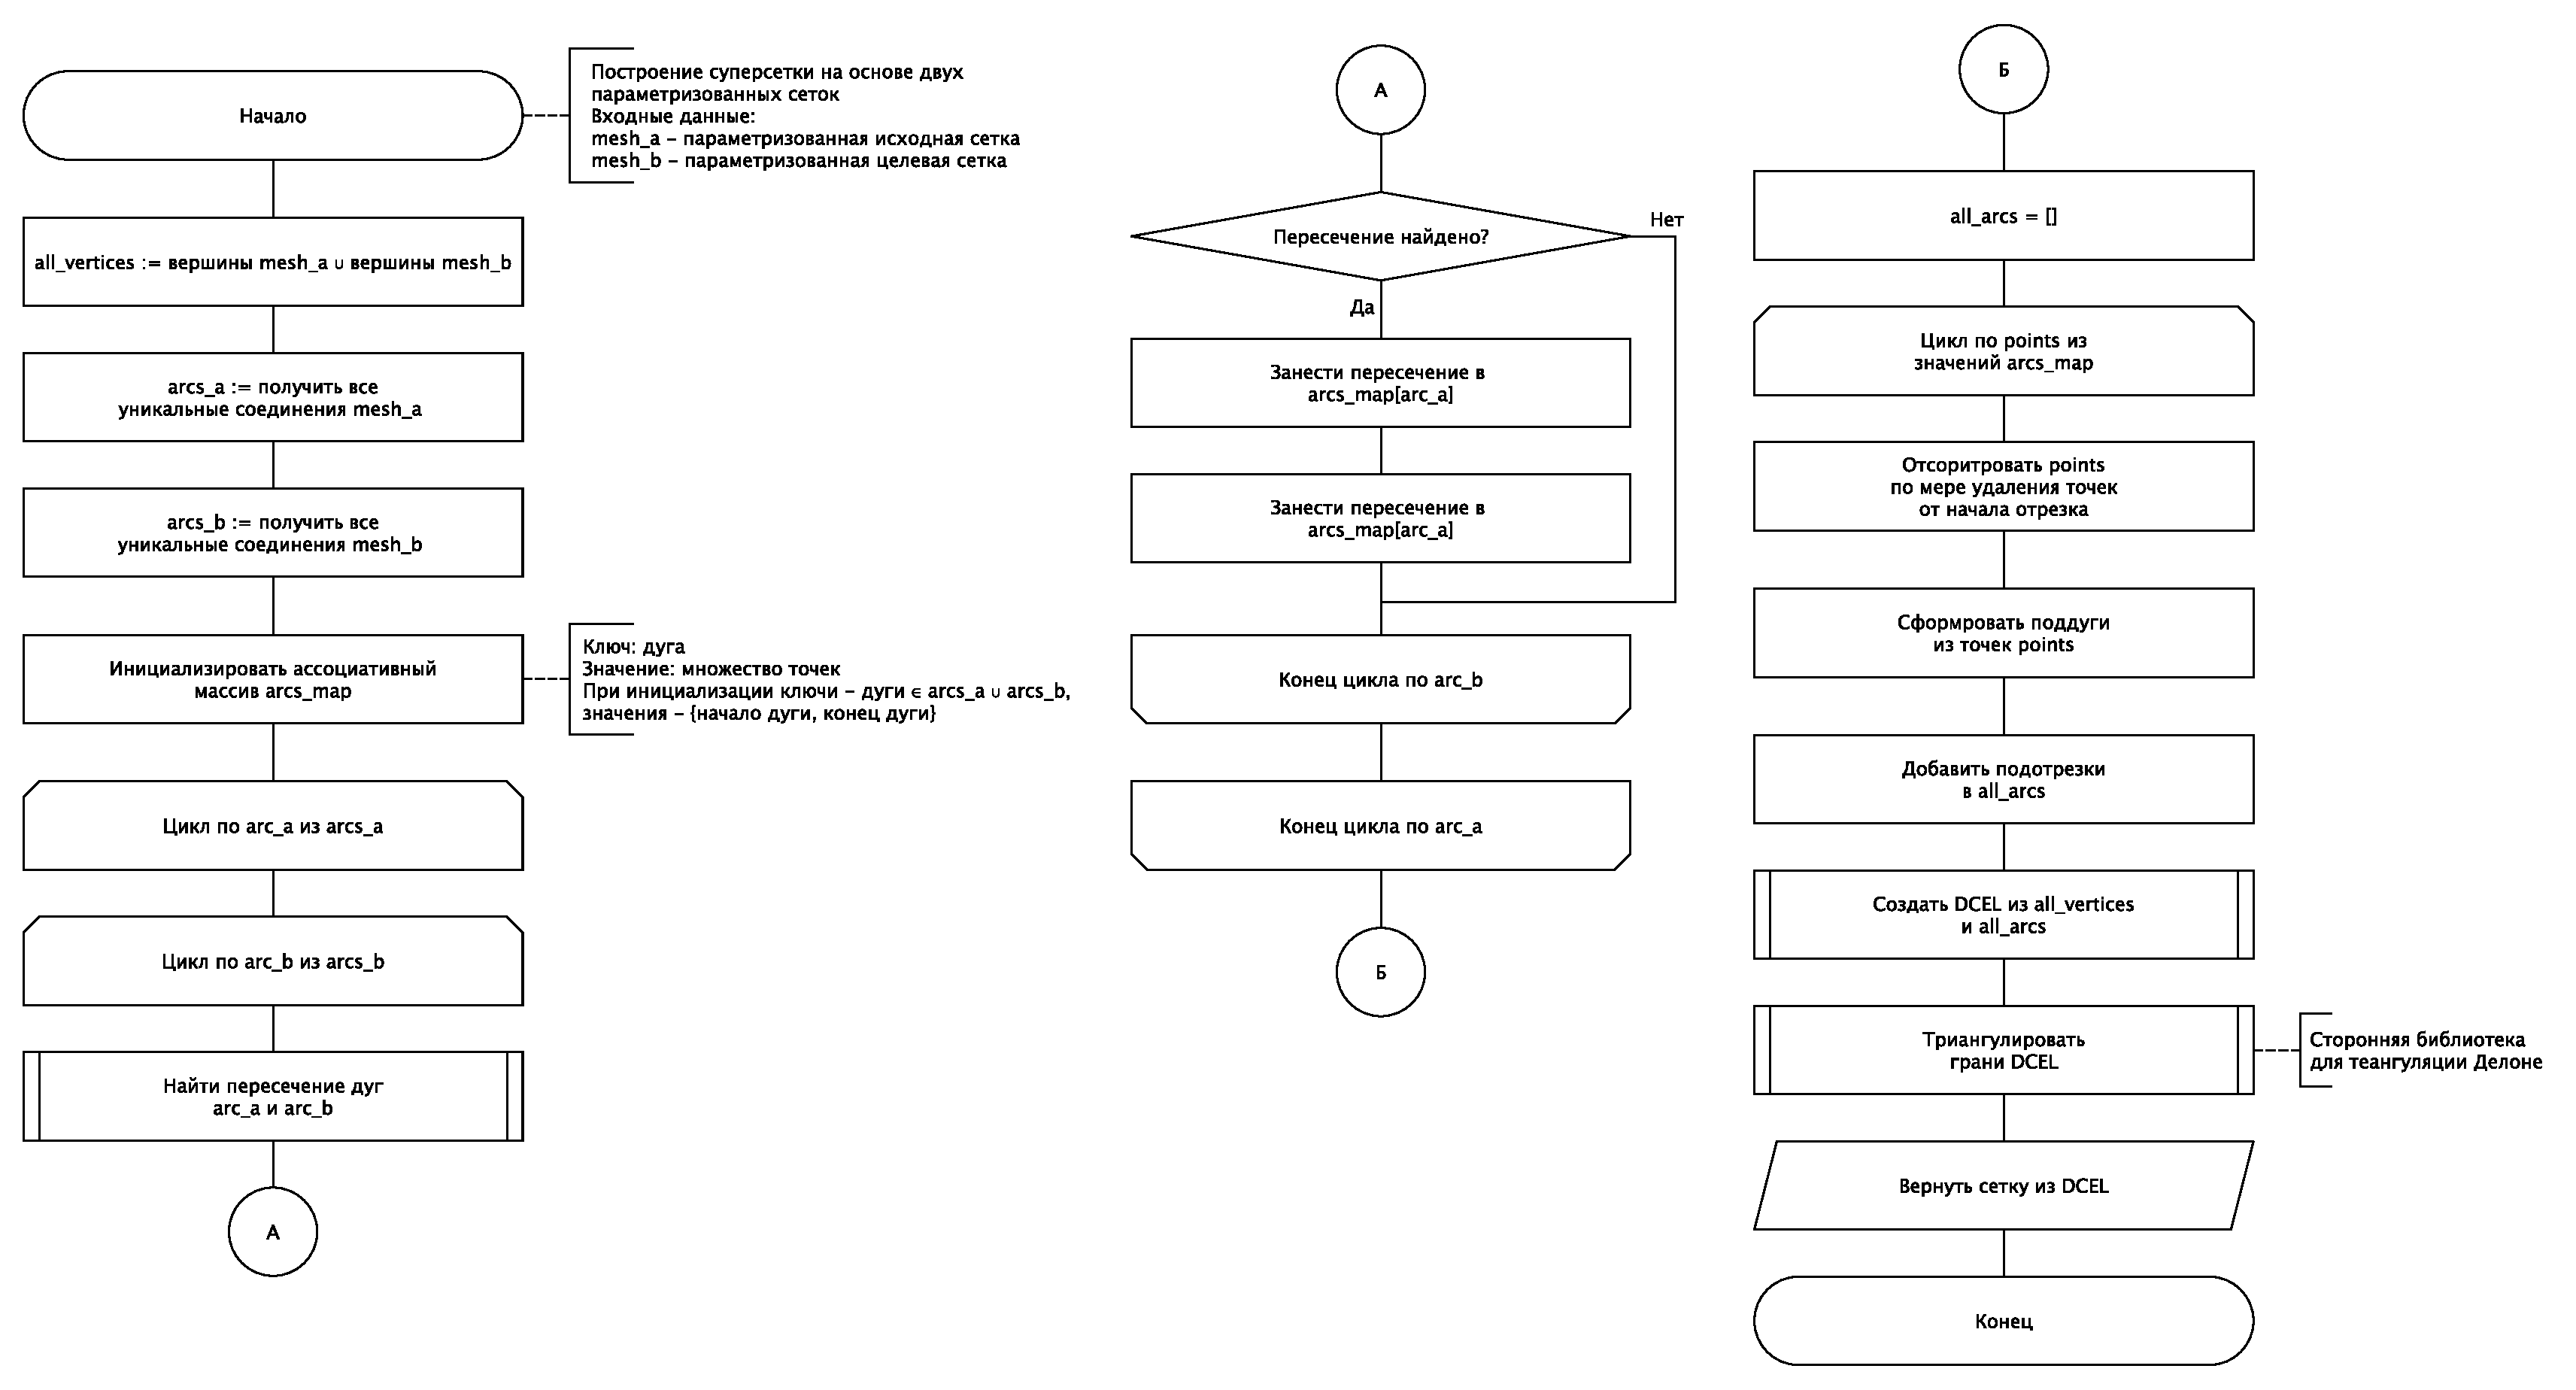
\includegraphics[width=\textwidth]{flowchart_bulid_supermesh}
    \caption{Схема алгоритма построения суперсетки на единичной сфере}
    \label{fig:flowchart_build_supermesh}
\end{figure}

\begin{figure}[H]
    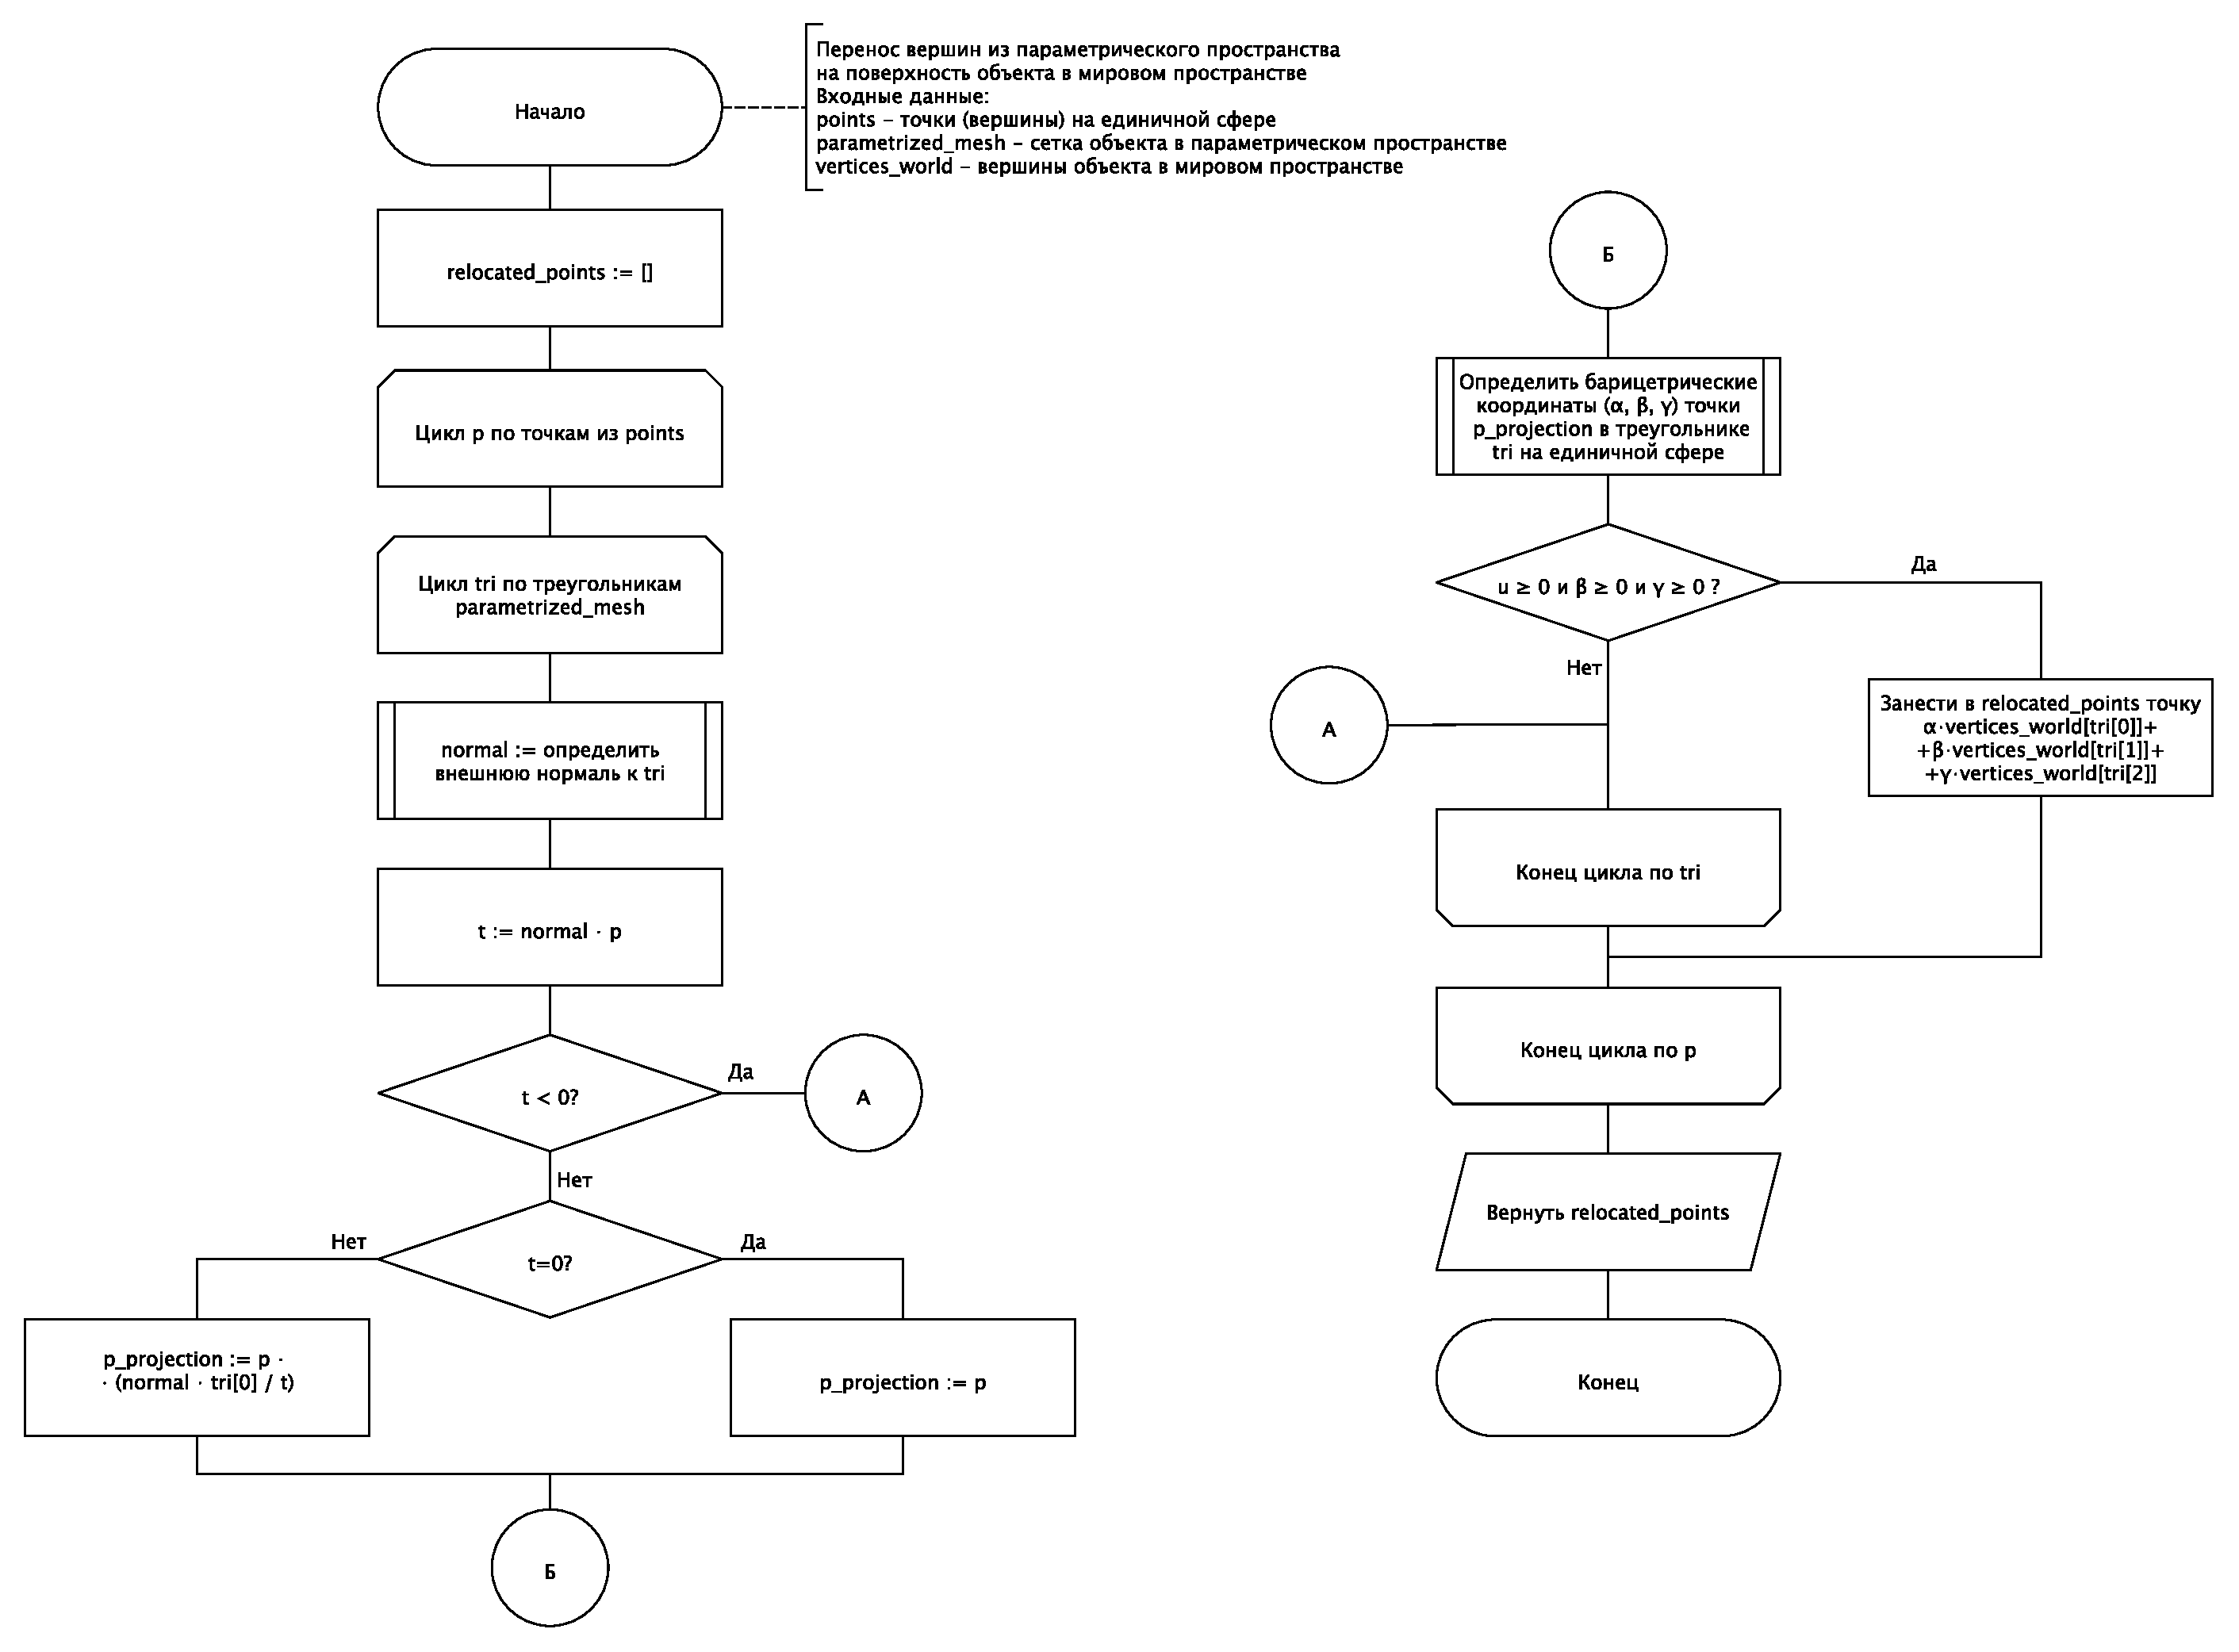
\includegraphics[width=\textwidth]{flowchart_vertex_relocation}
    \caption{Схема алгоритма вычисления положения вершин суперсетки на поверхности объекта по их параметрическим координатам}
    \label{fig:flowchart_vertex_relocation}
\end{figure}

\begin{figure}[H]
    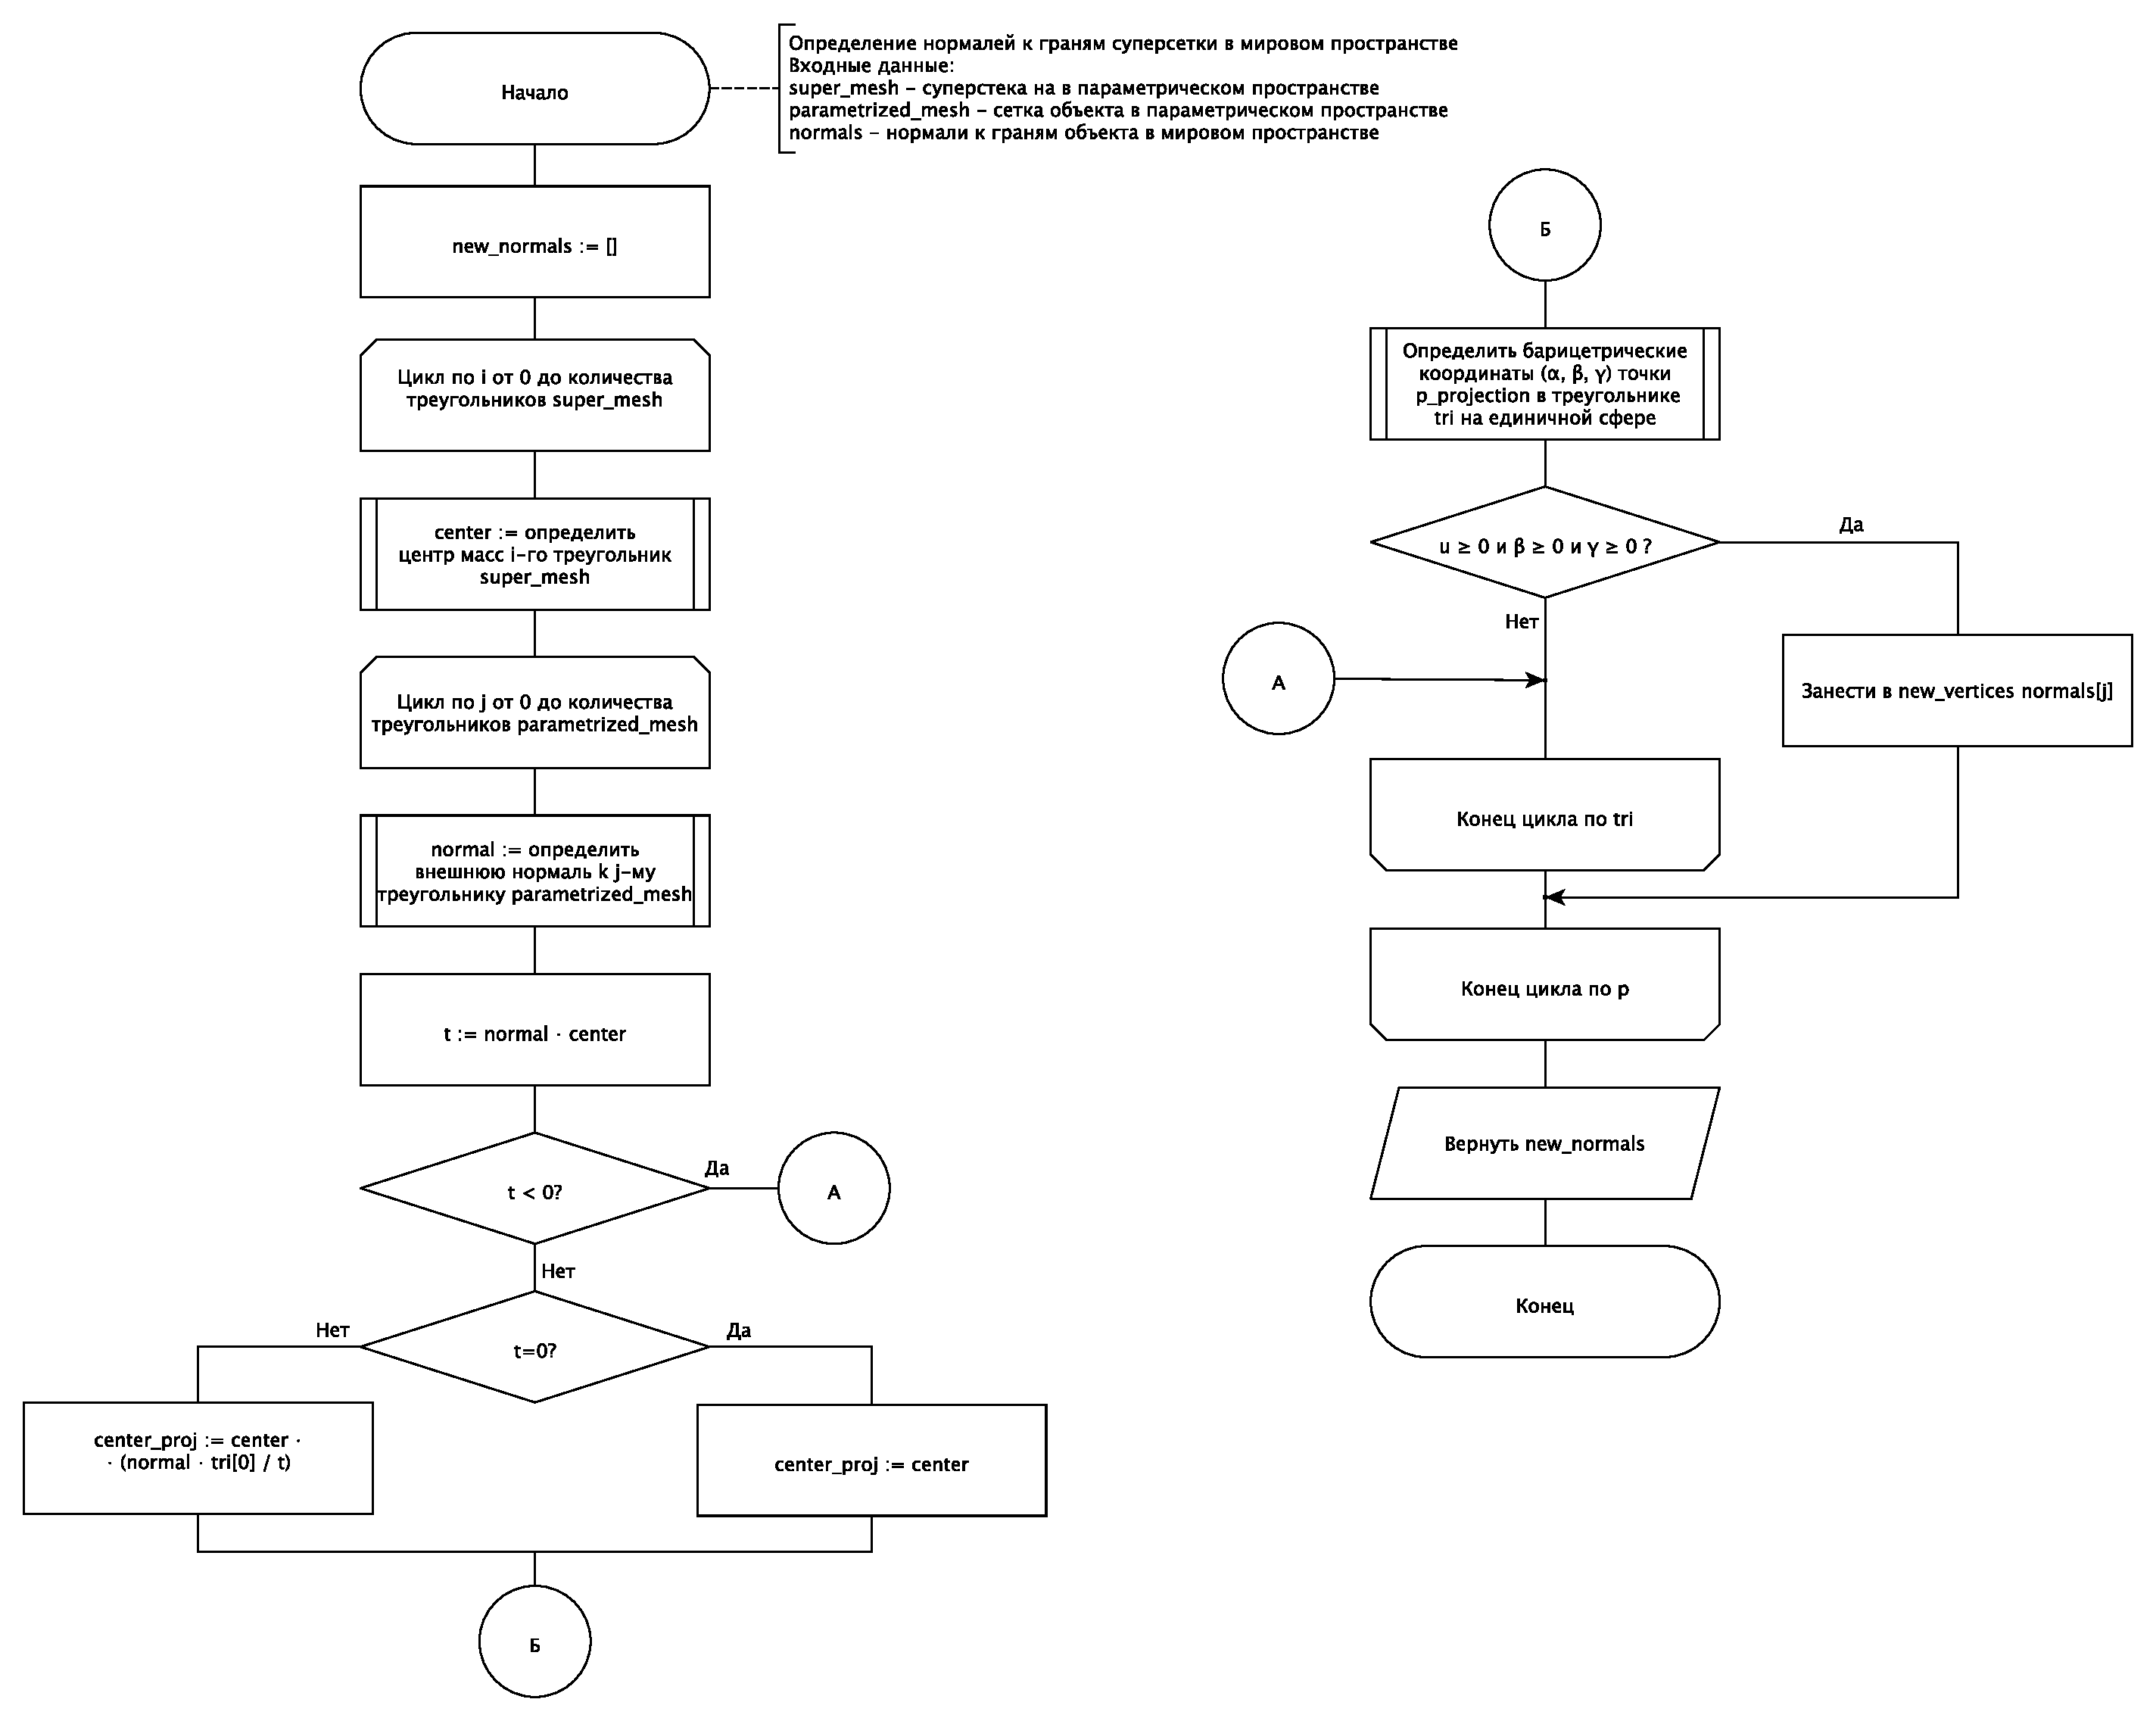
\includegraphics[width=\textwidth]{flowchart_normals_relocation}
    \caption{Схема алгоритма определения нормалей к граням суперсетки на основе соответствия с сетокой объекта в параметрическом пространстве}
    \label{fig:flowchart_normals_relocation}
\end{figure}

\section{Математические основы алгоритмов}

\subsection{Барицентрические координаты}

Барицентрические координаты $\alpha$, $\beta$ и $\gamma$ определяют положение точки $P$ относительно вершин треугольника $A$, $B$ и $C$~\cite{foley}.

Точка $P$ находится внутри или на границах треугольника $ABC$, если она может быть представлена в виде аффинной комбинации вершин~\cite{foley}:
\begin{equation}
    P = \alpha A + \beta B + \gamma C \text{, где } \alpha + \beta + \gamma = 1, \text{ и } \alpha, \beta, \gamma \geq 0~\text{\cite{foley}}
\end{equation}

Если хотя бы одна из координат $\alpha, \beta, \gamma$ отрицательна, то точка $P$ лежит вне треугольника~\cite{foley}.

Барицентрическая координата $\alpha$ точки $P$ пропорциональна площади треугольника $PBC$ (см. рисунок~\ref{fig:barycentric}) (треугольника, противолежащего вершине $A$)~\cite{foley}.

\begin{figure}[H]
    \centering
    \includegraphics[width=0.5\textwidth]{barycentric_coordinates}
    \caption{Точка $P$ разделяет треугольник $ABC$ на три меньших треугольника, площади которых соотносятся как $\alpha$, $\beta$ и $\gamma$; Барицентрические координаты точки $P$ равны ($\alpha$, $\beta$, $\gamma$)~\cite{foley}}
    \label{fig:barycentric}
\end{figure}

Координата $\alpha$ точки $P$ определяется как отношение площади треугольника $PBC$ к площади всего треугольника $ABC$~\cite{foley}:

\begin{equation}
    \alpha = \frac{S_{\triangle PBC}}{S_{\triangle ABC}}
\end{equation}

Аналогичные соотношения используются для $\beta$ (пропорционально $S_{\triangle PAC}$) и $\gamma$ (пропорционально $S_{\triangle PAB}$).

На плоскости барицентрические координаты точки $P$ в треугольнике $ABC$ могут быть вычислены при помощи косого произведения:

\begin{equation}
    \begin{aligned}
        \begin{cases}
            \alpha = \frac{|BC \times BP|}{|AB \times AC|} = \frac{(C - B)_x \cdot (P - B)_y - (C - B)_y \cdot (P - B)_x}{(B - A)_x \cdot (C - A)_y - (B - A)_y \cdot (C - A)_x} \\
            \beta = \frac{|CA \times CP|}{|AB \times AC|} = \frac{(A - C)_x \cdot (P - C)_y - (A - C)_y \cdot (P - C)_x}{(B - A)_x \cdot (C - A)_y - (B - A)_y \cdot (C - A)_x} \\
            \gamma = 1 - \alpha - \beta
        \end{cases}
    \end{aligned}
\end{equation}

\subsection{Поиск пересечения дуг на единичной сфере}

Для нахождения пересечения дуг необходимо:
\begin{enumerate}
    \item[1)] найти прямую по которой пересекаются плоскости, содержащие дуги;
    \item[2)] найти точки пересечение прямой с единичной сферой;
    \item[3)] проверить принадлежность точек обеим дугам.
\end{enumerate}

Пусть дуга $A$ задана радиус-векторами $\mathbf{A_0}$ и $\mathbf{A_1}$, а дуга $B$~--- векторами $\mathbf{B_0}$ и $\mathbf{B_1}$. Нормали к плоскостям, содержащим дуги, вычисляются согласно~\eqref{eq:arc_normals}:
\begin{equation}
    \label{eq:arc_normals}
    \begin{cases}
        \mathbf{n_A} = \mathbf{A_0} \times \mathbf{A_1} \\
        \mathbf{n_B} = \mathbf{B_0} \times \mathbf{B_1}
    \end{cases}
\end{equation}

Направляющий вектор $\mathbf{d}$ прямой их пересечения равен векторному произведению нормалей, как показано в~\eqref{eq:dir_vector}:
\begin{equation}
    \label{eq:dir_vector}
    \mathbf{d} = \mathbf{n_A} \times \mathbf{n_B} = (\mathbf{A_0} \times  \mathbf{A_1}) \times (\mathbf{B_0} \times  \mathbf{B_1})
\end{equation}

Радиус-векторы точек-кандидатов, полученные пересечением этой прямой с единичной сферой, определяются по формуле~\eqref{eq:candidate_points}:
\begin{equation}
    \label{eq:candidate_points}
    \mathbf{P}_{1,2} = \pm \frac{\mathbf{d}}{\|\mathbf{d}\|}
\end{equation}

Точка $\mathbf{P}$ лежит на дуге $\mathbf{A_0A_1}$ тогда и только тогда, когда сумма сферических расстояний от концов дуги до точки равна длине самой дуги. На единичной сфере, где радиус-векторы точек единичны, сферическое расстояние равно углу между векторами и вычисляется через арккосинус их скалярного произведения.

Следовательно, одна из точек $\mathbf{P}$, найденных в~\eqref{eq:candidate_points}, является пересечением, если для нее выполняются условия~\eqref{eq:arc_intersect}:
\begin{equation}
    \label{eq:arc_intersect}
    \begin{cases}
        \arccos{(\mathbf{A_0} \cdot \mathbf{P})} + \arccos{(\mathbf{P} \cdot \mathbf{A_1})} \leqslant \arccos{(\mathbf{A_0} \cdot \mathbf{A_1})} \\
        \arccos{(\mathbf{B_0} \cdot \mathbf{P})} + \arccos{(\mathbf{P} \cdot \mathbf{B_1})} \leqslant \arccos{(\mathbf{B_0} \cdot \mathbf{B_1})}
    \end{cases}
\end{equation}

\subsection{Поиск точки внутри объекта}
Основные шаги:
\begin{enumerate}
    \item[1)] Испустить луч из центра масс $O$ любой грани в направлении внутренней нормали.
    \item[2)] Найти все точки пересечения с другими гранями.
    \item[3)] Определить ближайшую к началу луча точку пересечения $I$.
    \item[4)] Вернуть точку по середине отрезка $OI$.
\end{enumerate}

\subsubsection{Пересечение луча с полигоном}
В параметрическом представлении луча задается уравнением~\eqref{eq:ray-param}.
\begin{equation}
    \label{eq:ray-param}
    P(t) = P_0 + \mathbf{d} \cdot t,
\end{equation}

где $P_0$ --- начальная точка луча; $\mathbf{d}$ --- направляющий вектор луча.

Произвольная точка $M$ лежит на плоскости $A$, если для нее выполняется равенство~\eqref{eq:plane}.

\begin{equation}
    \label{eq:plane}
    (M - M_A) \cdot \mathbf{n_A} = 0,
\end{equation}

где $M$ --- произвольная точка \\
$M_A$ --- известная точка на плоскости $A$\\
$\mathbf{n_A}$ --- вектор нормали к $A$.

После подстановки~\eqref{eq:ray-param} в~\eqref{eq:plane}, получилось уравнение~\eqref{eq:t-intersect} для нахождения параметра $t$ точки пересечения луча с плоскостью полигона.

\begin{equation}
    \label{eq:t-intersect}
    t = \frac{(M_A - P_0) \cdot \mathbf{n_A}}{\mathbf{d} \cdot \mathbf{n_A}}
\end{equation}

Если знаменатель $\mathbf{d} \cdot \mathbf{n_A}$ равен нулю, то луч параллелен плоскости полигона. Если $t < 0$, то пересечение находится позади начала луча, и такая точка отбрасывается, так как поиск ведется внутри объекта.

Найдя точку пересечения луча с плоскостью, необходимо определить, лежит ли она внутри полигона. Для этого можно использовать барицентрические координаты.

\subsection{Матрицы преобразований}

\subsubsection{Матрицы преобразований в мировое пространство}
Для перевода объектов из их локального пространства в мировое пространство используются матрицы масштабирования и поворота~\cite{foley, rogers, porev}.
Матрицы поворота вокруг осей $X$, $Y$ и $Z$ представлены в формулах~\eqref{eq:rot_x},~\eqref{eq:rot_y} и~\eqref{eq:rot_z} соответственно.

\begin{equation}
    \label{eq:rot_x}
    R_X(\theta) =
    \begin{pmatrix}
        1 & 0 & 0 & 0 \\
        0 & \cos\theta & -\sin\theta & 0 \\
        0 & \sin\theta & \cos\theta & 0 \\
        0 & 0 & 0 & 1
    \end{pmatrix}
\end{equation}

\begin{equation}
    \label{eq:rot_y}
    R_Y(\theta) =
    \begin{pmatrix}
        \cos\theta & 0 & \sin\theta & 0 \\
        0 & 1 & 0 & 0 \\
        -\sin\theta & 0 & \cos\theta & 0 \\
        0 & 0 & 0 & 1
    \end{pmatrix}
\end{equation}

\begin{equation}
    \label{eq:rot_z}
    R_Z(\theta) =
    \begin{pmatrix}
        \cos\theta & -\sin\theta & 0 & 0 \\
        \sin\theta & \cos\theta & 0 & 0 \\
        0 & 0 & 1 & 0 \\
        0 & 0 & 0 & 1
    \end{pmatrix}
\end{equation}

Матрица масштабирования представлена в формуле~\eqref{eq:scale}.

\begin{equation}
    \label{eq:scale}
    S =
    \begin{pmatrix}
        S_X & 0 & 0 & 0 \\
        0 & S_Y & 0 & 0 \\
        0 & 0 & S_Z & 0 \\
        0 & 0 & 0 & 1
    \end{pmatrix}
\end{equation}

%TODO: Возможно не стоит об этом писать
%\subsubsection{Матрица перспективной проекции}
%
%\begin{equation}
%    \label{eq:perspective}
%    M =
%    \begin{bmatrix}
%        \frac{\ctg{\frac{FOV_y}{2}}}{aspect} & 0 & 0 & 0 \\
%        0 & \ctg{\frac{FOV_y}{2}} & 0 & 0 & 0 \\
%        0 & 0 & -\frac{Z_{far} + Z_{near}}{Z_{far} - Z_{near}} & -1 \\
%        0 & 0 & -2\frac{Z_{far} \cdot Z_{near}}{Z_{far} - Z_{near}} & 0
%    \end{bmatrix}
%\end{equation}

\section*{Вывод}

В данном разделе была приведена функциональная схема морфинга, разработаны и представлены схемы основных алгоритмов и их математические основы.

\clearpage